Traditional networking method requires network administrators to configure each and every individual switches manually since each switches have configuration API that is vendor specific. As cloud services are becoming more ubiquitous, the traditional method become more costly which led to a push for software defined networking (SDN). SDN unifies the API needed to control all switches through a single controller which allows dynamic control over the network. However, it can also lead to security issues not faced before in the traditional networking.

% discuss the security aspect from the work: Towards Secure and Dependable SDN

% ==========================================================================

In this paper, we will define \textit{firewall bypass threat} as defined by Zhang et al.\cite{}: constructions of flow tables such that existence of a flow is possible against the firewall policy.
The bypass exploits the fact that switches query the controller only when unspecified flow is about to enter the network.
Figure \ref{fig:firewall_bypass} from \cite{} shows an example of an instance when the by pass can occur.
As shown in the picture, flow from $A$ to $C$ is restricted by firewall policy.
However, the switches are not aware of the policy.
Therefore, incremental modifications to the flow tables can be made to cause policy conflict.
In this case, a packet with source set to $A$ and destination set to $B$ gets the source header modified to $D$ in the first switch.
In the second switch, the second switch modifies the destination from $B$ to $C$.
As a result, a packet which originally meant to go from $A$ to $B$ ends up going from $A$ to $C$.

There are three primary aspects to solve this problem:
policy conflict detection, policy conflict resolution, and scalability.
Policy conflict detection methods detects policies that goes against the firewall policy in network applications.
Policy conflict resolution decides which action to take when the conflict is detected.
The resolution methods are non-trivial since the actions may differ depending on the purpose the SDN serves.
And finally, scalability which deals with how scalable the solution is in terms of increasing the size of SDN controlled by a single controller or increasing the number of controllers.


Therefore the paper is structured as follows.
In the next section, I provide an overview of how SDN is constructed.
Then, I present papers with emphasis on the three primary aspectes of the solution where each aspect is preseted per chapter.
Finally, I provide a summary of the papers reviewed and a conclusion.

\begin{figure}[t]
  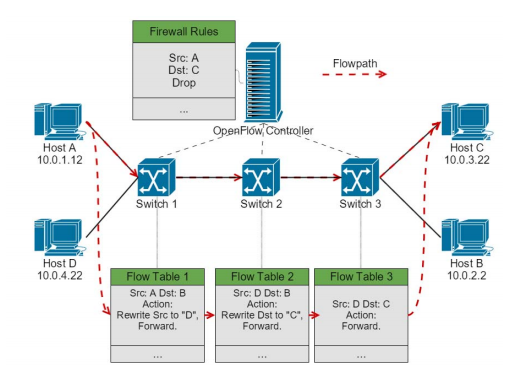
\includegraphics[width=\linewidth]{firewall_bypass.png}
  \caption{This figure is from Zhang et al. \cite{} which shows how firewall bypass can occur.}
  \label{fig:firewall_bypass}
\end{figure}
